% Path: docs/report_final.tex
\documentclass[11pt,a4paper]{article}

\usepackage[utf8]{inputenc}
\usepackage[T1]{fontenc}
\usepackage{geometry}
\usepackage{booktabs}
\usepackage{graphicx}
\usepackage{float}
\usepackage{hyperref}
\usepackage{enumitem}

\geometry{margin=1in}

\title{CNN-LSTM Image Captioning on Flickr8k}
\author{Giuseppe Dimonte}
\date{\today}

\begin{document}

\maketitle

\begin{abstract}
This report presents the implementation and evaluation of a CNN-LSTM image captioning system trained on Flickr8k. The project includes caption preprocessing, vocabulary construction, supervised training, BLEU-based evaluation, and qualitative analysis. Four configurations were compared in a controlled setting: a baseline model, an ablation without scheduled sampling, an ablation without label smoothing, and a fine-tuned model. The best result was obtained by the fine-tuned configuration, which achieved a BLEU-4 score of 0.0649, outperforming the baseline BLEU-4 score of 0.0472.
\end{abstract}

\section{Introduction}

Image captioning is a multimodal learning problem in which a system receives an image as input and produces a natural language description as output. The task requires both visual understanding and sequence generation, and it is therefore naturally formulated as an image-to-sequence problem.

The assignment required the implementation of a CNN-LSTM architecture on the Flickr8k dataset. In the final project, a pretrained convolutional encoder extracts compact image features, and an LSTM decoder generates captions word by word. The work covers the entire pipeline from preprocessing to evaluation and compares multiple training configurations under a controlled experimental protocol.

\section{Dataset and Preprocessing}

The experiments were performed on Flickr8k, a dataset in which each image is associated with five reference captions. The preprocessing stage was designed to match the assignment requirements:
\begin{itemize}[leftmargin=*]
    \item lowercase conversion;
    \item punctuation removal;
    \item digit removal;
    \item removal of single-letter words;
    \item vocabulary construction with special tokens.
\end{itemize}

The final prepared artifacts were:
\begin{itemize}[leftmargin=*]
    \item \texttt{data/vocab.json}
    \item \texttt{data/Flickr8k\_text/train.csv}
    \item \texttt{data/Flickr8k\_text/val.csv}
    \item \texttt{data/Flickr8k\_text/test\_captions.json}
\end{itemize}

Observed sizes after preprocessing:
\begin{itemize}[leftmargin=*]
    \item 30000 training caption rows
    \item 5000 validation caption rows
    \item 1000 test images
    \item vocabulary size: 2985 tokens
\end{itemize}

\section{Model}

The implemented system follows a classical encoder-decoder design:
\begin{itemize}[leftmargin=*]
    \item \textbf{Encoder}: pretrained InceptionV3
    \item \textbf{Decoder}: single-layer LSTM
    \item \textbf{Output layer}: linear projection from hidden state to vocabulary logits
\end{itemize}

The training code includes:
\begin{itemize}[leftmargin=*]
    \item scheduled sampling
    \item label smoothing
    \item gradient clipping
    \item checkpoint saving
    \item checkpoint resume
    \item BLEU-1 to BLEU-4 evaluation with 5 references per image
\end{itemize}

\section{Experimental Setup}

All experiments were run in the \texttt{captioning} environment using PyTorch \texttt{2.9.1+cpu}. The device used for training and evaluation was CPU.

Four configurations were compared:
\begin{enumerate}[leftmargin=*]
    \item \textbf{Baseline}
    \item \textbf{No Scheduled Sampling}
    \item \textbf{No Label Smoothing}
    \item \textbf{Fine-tuning}
\end{enumerate}

In the final comparison, all four experiments were run for 5 epochs.

\section{Quantitative Results}

\begin{table}[H]
\centering
\caption{BLEU comparison across the final experiments.}
\begin{tabular}{lcccc}
\toprule
Experiment & BLEU-1 & BLEU-2 & BLEU-3 & BLEU-4 \\
\midrule
Baseline & 0.2553 & 0.1556 & 0.0928 & 0.0472 \\
No Scheduled Sampling & 0.2232 & 0.1242 & 0.0717 & 0.0396 \\
No Label Smoothing & 0.2404 & 0.1435 & 0.0809 & 0.0394 \\
Fine-tuning & 0.3301 & 0.2022 & 0.1189 & 0.0649 \\
\bottomrule
\end{tabular}
\end{table}

\begin{table}[H]
\centering
\caption{Training summary of the final experiments.}
\begin{tabular}{lccc}
\toprule
Experiment & Best Val Loss & Final Train Loss & Final Val Loss \\
\midrule
Baseline & 4.1927 & 4.8016 & 4.2332 \\
No Scheduled Sampling & 4.0106 & 3.5373 & 4.0234 \\
No Label Smoothing & 3.5029 & 4.0860 & 3.5738 \\
Fine-tuning & 3.6614 & 4.7512 & 4.2861 \\
\bottomrule
\end{tabular}
\end{table}

\section{Discussion}

The ablation study shows that both scheduled sampling and label smoothing improve caption quality. Removing either of them lowers all BLEU scores relative to the baseline.

The most important result is obtained with CNN fine-tuning. The fine-tuned model achieves the strongest BLEU scores across all metrics, with BLEU-4 improving from 0.0472 in the baseline to 0.0649. This indicates that adapting the visual encoder to the captioning task provides a measurable benefit.

An important observation is that lower training loss does not always imply better caption quality. In particular, the configuration without scheduled sampling obtains a lower training loss than the baseline, but worse BLEU scores. This is a relevant result because it highlights the difference between fitting the training distribution and generalizing during autoregressive generation.

\section{Qualitative Analysis}

\begin{figure}[H]
    \centering
    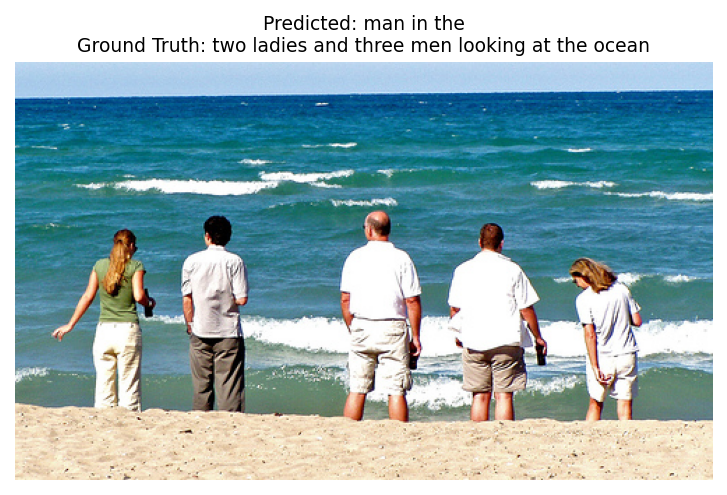
\includegraphics[width=0.8\textwidth]{selected_figures/baseline_example.png}
    \caption{Representative baseline output. The predicted caption is simple and partially correct, but it remains generic and incomplete relative to the reference caption.}
    \label{fig:baseline_example}
\end{figure}

\begin{figure}[H]
    \centering
    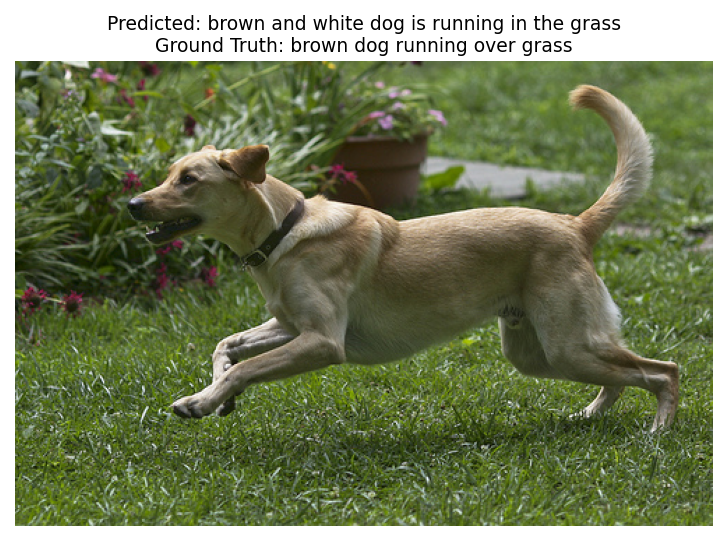
\includegraphics[width=0.8\textwidth]{selected_figures/finetune_example.png}
    \caption{Representative fine-tuned output. The prediction correctly identifies the main object and action, and is more precise than the baseline outputs.}
    \label{fig:finetune_example}
\end{figure}

\begin{figure}[H]
    \centering
    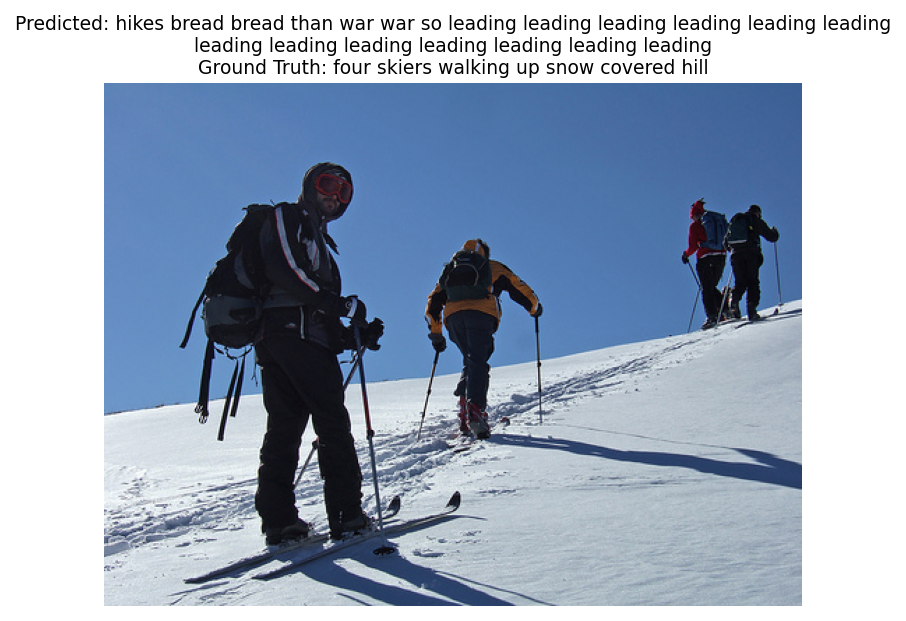
\includegraphics[width=0.8\textwidth]{selected_figures/failure_case.png}
    \caption{Failure case. The generated sentence is repetitive and semantically incorrect, showing that the model can still collapse into unstable outputs on more difficult scenes.}
    \label{fig:failure_case}
\end{figure}

\section{Limitations}

\begin{itemize}[leftmargin=*]
    \item All experiments were executed on CPU, which significantly increased training time.
    \item Flickr8k is relatively small for image captioning and limits the absolute quality of the generated outputs.
    \item The project focuses on a CNN-LSTM architecture and does not include transformer-based captioning models.
\end{itemize}

\section{Conclusion}

This project implemented a complete CNN-LSTM image captioning pipeline on Flickr8k, from preprocessing to evaluation. The final experiments show that scheduled sampling and label smoothing both contribute positively to caption generation quality, while CNN fine-tuning yields the best final results. The repository now contains reproducible preprocessing scripts, saved checkpoints, experimental logs, BLEU results, and qualitative figures, making the work suitable for final academic presentation.

\section*{Available Artifacts}

The following files support the final report:
\begin{itemize}[leftmargin=*]
    \item \texttt{results/metrics\_summary.csv}
    \item \texttt{results/experiment\_summary.csv}
    \item \texttt{results/*\_predictions.json}
    \item \texttt{logs/*}
    \item \texttt{figures/*}
    \item \texttt{LAB\_LOG.md}
\end{itemize}

\end{document}
